\NeedsTeXFormat{LaTeX2e}
\documentclass[11pt]{article}
%Absaetze nicht einruecken:
\usepackage{parskip}
\usepackage[utf8]{inputenc}
\usepackage[T1]{fontenc}
\usepackage{ae}
\usepackage[intlimits, sumlimits, namelimits]{amsmath}
\usepackage{bbm}
%Neue Macros fuer Mathe:
%in parentheses - gleich mit richtiger Groesse
\newcommand{\inp}[1]{\ensuremath{\left(#1\right)}}
\newcommand{\sqr}{\ensuremath{^{2}}}
\newcommand{\cube}{\ensuremath{^{3}}}
%Mengensymbole mit doppelten senkrechten Strichen:
\newcommand{\set}[1]{\ensuremath{\mathbbm{#1}}}
%definiert eine Norm, also zwei senkrechte Striche auf jeder Seite:
\newcommand{\norm}[1]{\ensuremath{\left|#1\right|}}
\newcommand{\vect}[2]{\ensuremath{\inp{\hspace{-.8ex}\begin{array}{c}#1\\#2\end{array}\hspace{-.4ex}}}}
%\newcommand{\vec3}[3]{\ensuremath{\inp{\hspace{-.8ex}\begin{array}{r}#1\\#2\\#3\end{array}\hspace{-.4ex}}}}
\newcommand{\entspr}{\ensuremath{\,\,\hat{=}\,\,}}%
\newcommand{\dx}[1][x]{\ensuremath{\textnormal d #1}}

\newcommand{\ta}{\tilde \alpha}

% For stupid thinkos:
\newcommand{\cross}{\times}

% Tabellen:
\usepackage{array}
\setlength{\extrarowheight}{.2mm}
%Links im Text:
\usepackage{hyperref}
\usepackage{graphics,graphicx,fancyvrb}
%Raender einstellen
%\usepackage[a4paper, left=25mm, right=5mm, top=30mm]{geometry}
\usepackage[a4paper]{geometry}
%Kopf - und Fusszeilen
\usepackage{lastpage}
\usepackage{fancyhdr}
	\lhead{Moritz Lenz}
	\chead{\bfseries{-- \thepage\ --}}
	\rhead{\thetitle}
	\lfoot{}
	\rfoot{}
	\cfoot{}
	\pagestyle{fancy}
\pagestyle{empty}

\sffamily

%Kopfzeile

\author{Moritz Lenz}
\title{Spintronics}
\begin{document}
\maketitle

This is an attempt to reproduce what Khodas wrote in {\em Spin 
Polarization of Nonmagnetic Heterostructures: The Basics of Spin
Optics}, PRL 92.086602.

\begin{figure}
    \begin{center}
        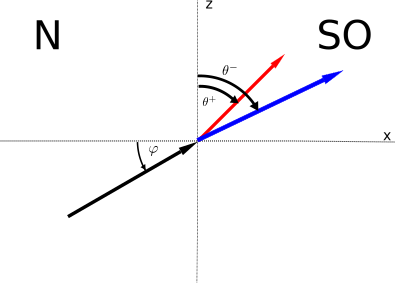
\includegraphics{setup-simple.pdf}
    \end{center}
    \label{fig:setup-zero}
    \caption{Scheme of the interface between normal (N)
            and spin-orbit (SO) regime}
\end{figure}

The setup consists of a 2D electron gas in the $x-z$ plane, where the
strength of the spin orbit interaction is a step function in $x$:
$\alpha(x) = \alpha \Theta(x)$. The region $x < 0$ is called the
"normal region", abbreviated with N, and the region with $x > 0$ is
called the "spin orbit" region, abbreviated as SO (Fig.
\ref{fig:setup-zero}).


The Hamiltonian looks like this:

\begin{align}
    H_r &= \frac{p^2}{2m} + (-\vec y \times \vec \sigma) \cdot
            \alpha(x) \vec p\\ 
    p^2 &= p_x^2 + p_z^2
\end{align}

With the eigenvalues and the velocities

\begin{align}
    E_{\pm} &= \frac{p^2}{2m} \pm \alpha \\
    v_{\pm} &= \frac{\partial E_{\pm}}{\partial p} = \frac{p}{m} \pm \alpha
\end{align}

When a wave travels from the N to the SO region it's energy doesn't
change. Since its dispersion relation changes, the momentum must also
change. From here on when we write $p$ we mean the momentum in the N
region. The momentum in the SO region then follows as

\begin{align}
    \label{eq:pso}
    p_{SO}^{\pm} &= m v_F (\sqrt{1 + \ta^2} \mp \tilde \alpha) \\
    \tilde\alpha &= \frac{\alpha}{v_F}
\end{align}

$p_z$ is conserved at the interface.

Solving the eigenvalue equation leads us to the eigenvectors in the SO
region:

\begin{align*}
   \chi_{SO}^{\pm} &= \frac{1}{n_{SO}^{\pm}} 
                      \vect{-p_{x,SO}^{\pm} \pm p_{SO}^\pm}{p_z} \\
    (n_{SO}^{\pm})^2 &= (-p_{x,SO}^{\pm} \pm p_{SO}^\pm)^2 + p_z^2
\end{align*}

Where the lower index $x$ means that the value is projected onto the
$x$ axis. The angle between the $x$ axis and the momentum of the
incident wave is called $\phi$, so that $p_x = p \cos \phi$.

Note that in the N regime $H$ is a diagonal matrix, and the direction
of the eigenvectors can be chosen with some freedom. We pick
$\chi_N^{\pm} = \lim_{\alpha \mapsto 0} \chi_{SO}^{\pm}$ to ensure that
$<\chi_N^+|\chi_{SO}^+> = 1$ holds true at a vanishing interface.



The overall wave function consists of an incident wave, 
and reflected and transmitted part. In general the incident wave can
be decomposed into one with $+$ and one with $-$ chirality, which
propagate and scatter independently. Let's consider the incident $+$
wave:

\begin{align}
    \Psi^+ = e^{i p_z z} * \left\{
        \begin{array}{ll}
            e^{i p_x x} \chi_N^+ + e^{- i p_x x} (\chi_N^+ r_{++} +
                    \chi_N^- r_{-+})    & x < 0\\
            e^{i p_x^+ x} \chi_{SO}^+ t_{++} + e^{i p_x^- x}
            \chi_{SO}^- t_{-+}          & x > 0
        \end{array} \right.
\end{align}

The coefficient $r_{-+}$ is the amplitude with which the incident wave
of $+$ chirality is reflected into $-$ chirality etc. while $t$
coefficients stand for transmission coefficients.

Analog equations can be found for the incident wave with $-$ chirality
by changing all signs that appear either as a subscript or
superscript.

To obtain the values for these coefficients one has to solve the
boundary conditions at the interface. The wave function is continuous
and the current is conserved, so $\frac{\partial H}{p_x} \Psi$ is also
continuous.

\begin{align}
    \Psi_N|_{x = -0}    &= \Psi_{SO}|_{x = +0} \label{eq:continuous}\\
    \left.\frac{\hat p_x}{m} \Psi_N\right|_{x = -0}
                        &= \left. \left(\frac{\hat p_x}{m} -\alpha \sigma_z\right)
                                \Psi_{SO}\right|_{x = +0}
\end{align}

The second equation can be evaluated with $\hat p_x = -i \partial_x$
(assuming $\hbar = 1$, as done in the rest of the calculation) and
carrying out the derivation (and multiplied by $m$), yielding

\begin{align}
    p_x \chi_N^+ (1 - r_{++}) - p_x \chi_N^- r_{-+}
        =& p_x^+ \chi_{SO}^+ t_{++} + p_x^- \chi_{SO}^- t_{-+} \nonumber\\
         &   - m \alpha \left(  \sigma_z \chi_{SO}^+ t_{++}
                            + \sigma_z \chi_{SO}^- t_{-+} \right)
\end{align}

Dividing it by  $p_x = p \cos \phi$: 

\begin{align}
    \chi_N^+ (1 - r_{++}) - \chi_N^- r_{-+}
        =& \frac{p_x^+}{p_x} \chi_{SO}^+ t_{++} + \frac{p_x^-}{p_x} \chi_{SO}^- t_{-+} \nonumber\\
         &   - \frac{\ta}{\cos \phi} \left(\sigma_z \chi_{SO}^+
                 t_{++} + \sigma_z \chi_{SO}^- t_{-+} \right)
                                \label{eq:j_continuous}
\end{align}

Equations \ref{eq:continuous} and \ref{eq:j_continuous} can be
expanded in powers of $\ta$. In solutions expanded to the first
non-zero order each are

\begin{align}
    t_{++} &= 1 +
            \frac{\ta}{2}\left( \frac{1}{\cos^2\phi} - 1 \right)\\
    t_{-+} &= \frac{\ta^2}{4}\tan \phi \\
    r_{++} &= \frac{\ta}{2} \tan^2 \phi\\
    r_{-+} &= -\frac{\ta}{2} \tan \phi
\end{align}

And for the incident wave with $-$ chirality

\begin{align}
    t_{--} &= 1 - \frac{\ta}{2} \left( \frac{1}{\cos^2\phi} - 1 \right)\\
    t_{+-} &= O(\ta^3)\\
    r_{--} &= -\frac{\ta}{2} \tan^2 \phi\\
    r_{+-} &= -\frac{\ta}{2} \tan \phi
\end{align}

\begin{figure}[h!tp]
    \includegraphics[width=\textwidth]{zero-plus.pdf}
    \includegraphics[width=\textwidth]{zero-minus.pdf}
    \label{fig:trans-zero}
    \caption{Transmission and reflection coefficients for the
            incident beam with $+$ (upper) and $-$ (lower) chirality
            and $\ta = 0.1$}
\end{figure}

Figure \ref{fig:trans-zero} shows the transmission and reflection
coefficients as a function of the angle $\phi$ of the incident wave.

For increasing $\phi$ the angle of the transmitted beam with $+$
chirality, $\theta^+$ grows even faster. When $\theta^+ =
\frac{\pi}{2}$ no current flows anymore with $+$ chirality, and we
call the corresponding $\phi_c$ a critical angle. (Note that $t_{++}$
is not zero in that region, but since the wave doesn't propagate, no
current flows).

Since

\begin{align}
    \cos \phi       &= \frac{p_x}{p}\\
    \cos \theta^+   &= \frac{p_{x,SO}}{p_{SO}}\\
    \theta_c^+      &= \frac{\pi}{2}
\end{align}

it follows that

\begin{align}
    \phi_c          &= -\sin ^{-1}\left(a-\sqrt{a^2+1}\right)
\end{align}

\clearpage
\section{Generalization to two Spin-Orbit regions}

The system can be generalized to two regions with non-zero spin-orbit
coupling (SO1 and SO2).

\begin{figure}
    \begin{center}
        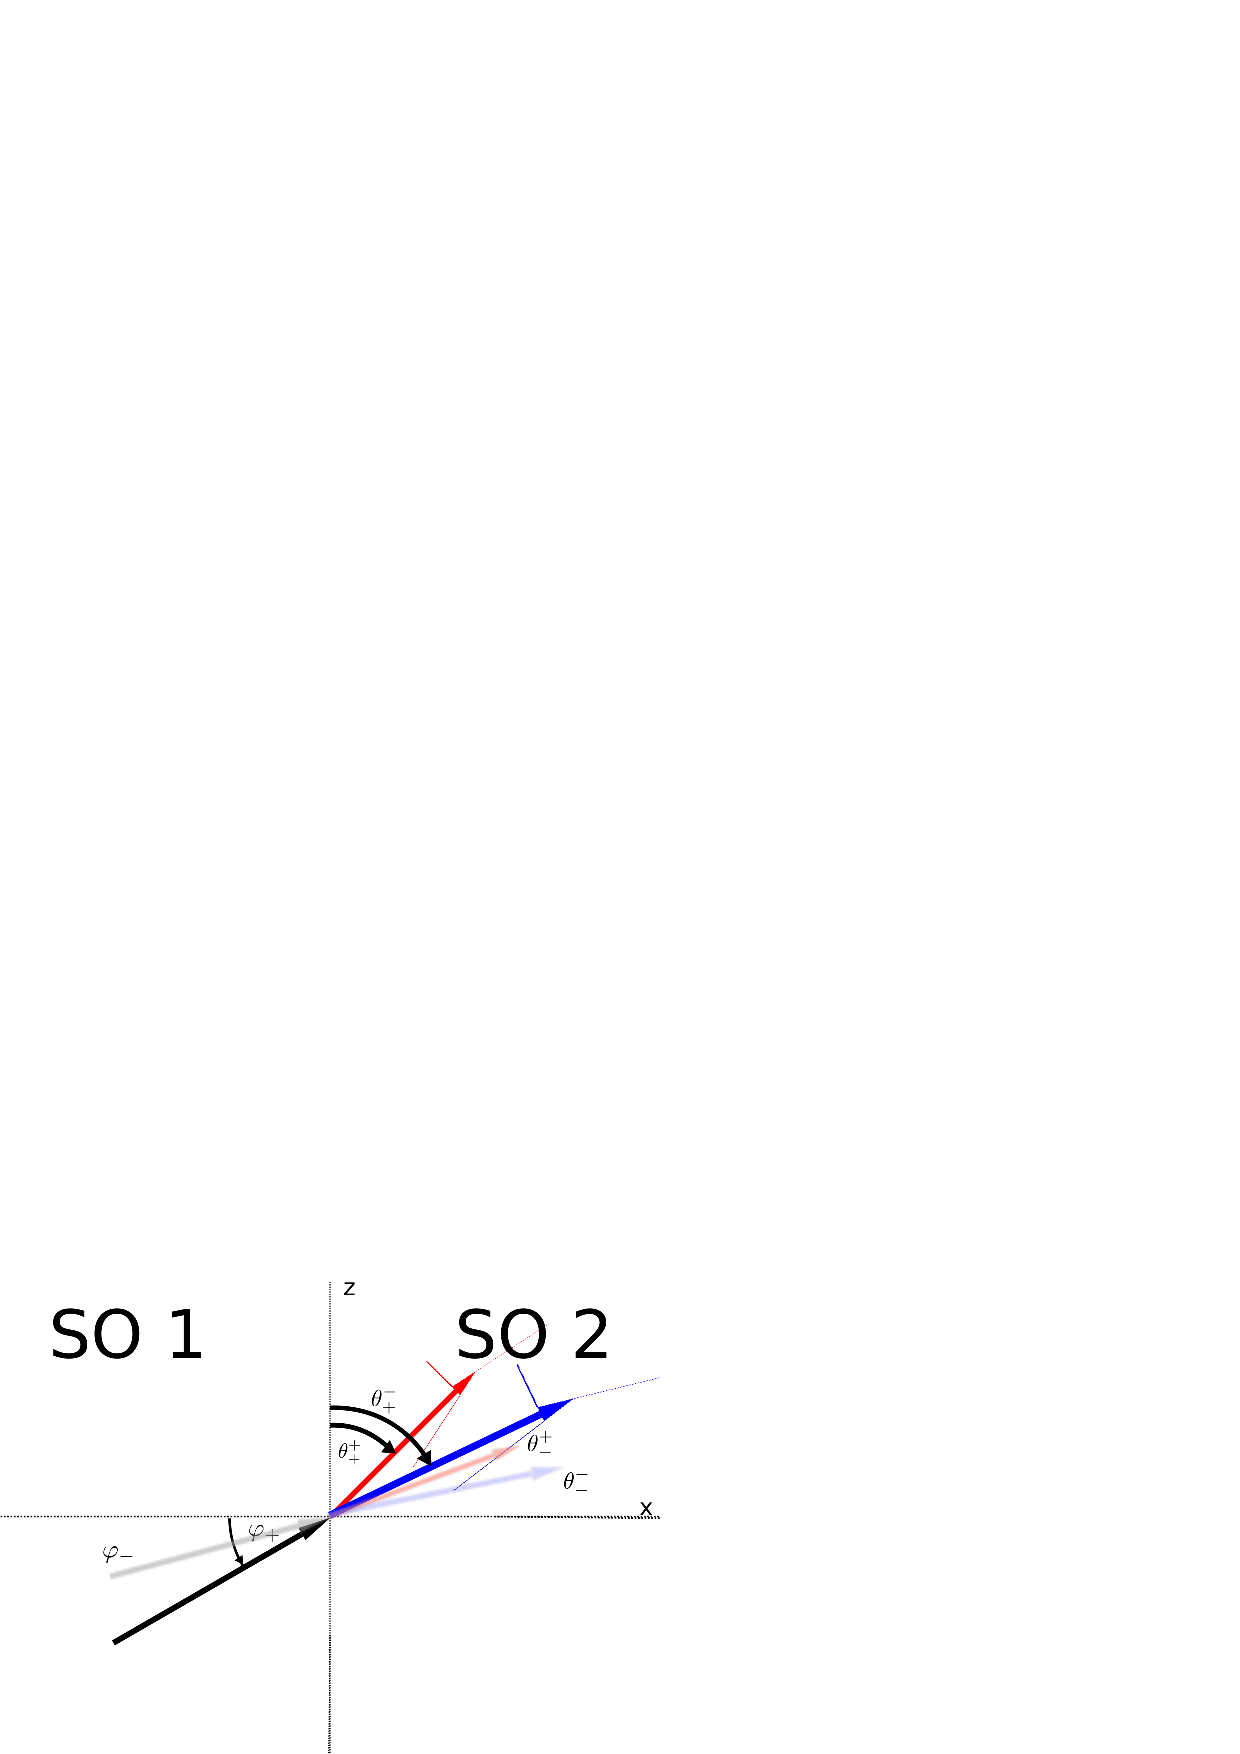
\includegraphics{setup-two-so-regions.pdf}
    \end{center}
    \label{fig:setup-nonzero}
    \caption{Scheme of the interface between two regions with
        different, non-zero spin orbit coupling}
\end{figure}

One just has to remember that the incident beam is split up
into two beams of different chirality, which propagate at different
angles. In general each beam is split up into two beams at the
interface, so there are up to four beams in SO2 region, two of each
chirality.

\end{document}

% vim: ts=4 sw=4 expandtab spell spelllang=en_us tw=70
